\section{Background}
\label{background}

This section presents the technical and mathematical background required to understand the report.

\subsection{Practical Byzantine Fault Tolerance (PBFT)}
Distributed systems are characterized by presence of independently failing components. Therefore fault tolerance is an important property for a distributed system that should remain available even in the presence of these failures. Derived from Byzanine General's problem\cite{bgp}, a system is Byzantine Fault Tolerant if it functions as desired even in the presence of malicious entities that can fail or pass incorrect information to other peers. It can be shown that in the presence of $f$ traitors, a byzantine fault tolerant system can exist only if the total number of generals is $>3f$. 

PBFT algorithm \cite{PBFT} provides a practical implementation for such a system through a 3-phase protocol: pre-prepare, prepare and commit. One active node of the system acts a primary and the rest act as backups.The primary receives the requests from the client and initiates the pre-prepare phase by broadcasting the message in the network. In the prepare every node broadcast authenticated messages in the network to signals its participation. After receiving $2f +1$ threshold prepare message, the nodes against broadcasts its commitment to the network. After receiving $2f +1$ commitments, the node accepts the message. We easily see that this requires $O(n^2)$ communication, therefore does not scale well. Further the consensus group is closed, making it unusable for open permission-less systems like crypto-currencies.

\subsection{BitCoin}
Bitcoin is digital currency introduced in 2009 on a decentralized peer-to-peer network. Without centralized authority, bitcoin operates on a public distributed ledger called blockchain. Bitcoin uses proof-of-work mechanism to achieve consensus among thousands of nodes. Miners are the participating nodes that mine for new blocks to append new transactions to the blockchain. New block must contain proof-of-work that solves a computationally difficult condition (eg: finding a nonce such that when hashed with the block content, it is smaller than some target) but is easily verifiable.
Due to its decentralized nature, a single malicious miner cannot attack the system. For a confirmed success, a 51\% attack on bitcoin is required which can cost over \$6 billion US dollars \cite{51}. However due to the probabilistic nature of Bitcoin's consensus, the consistency of a transaction is never guaranteed. Forks can occur in the blockchain which are resolved by the longest fork. Thus a committed transaction on a dissolved fork will be reverted. 


\subsection{Collective signing (CoSi)}
CoSi is protocol that performs efficient signing by multiple entities. Using Schnorr signatures, CoSi outputs a compact collective signature that is easily verifiable by the client.
CoSi protocol follows a tree-based communication to scale computation and communication. One round of CoSi protocol consists of four phases i.e. two communications round-trips:\\
1) Announcement: The root initiates the protocol by multicasting the message to be signed.\\
2) Commitment: Each node commits to a random secret and generates a public commit which it sends up the tree. On receiving all commitments, non-leaf nodes aggregate the commit before sending it up the tree.\\
3) Challenge: The leader multicasts a collective challenge down the tree.\\
4) Response: The nodes compute their response using their committed secret keys. They further aggregate the responses received from their children and send them further up the tree.
\begin{figure}[h]
	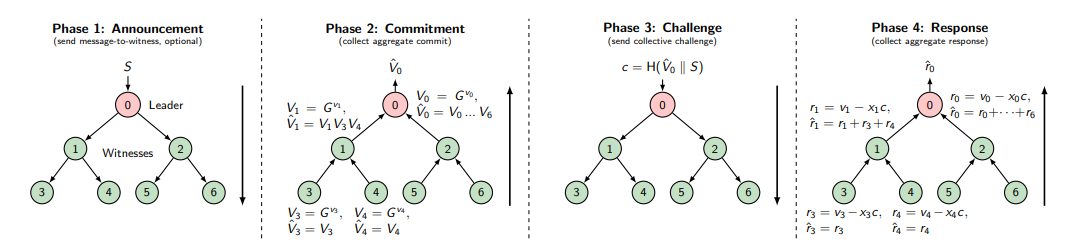
\includegraphics[width=14cm]{cosi.png}
	\caption{CoSi protocol with Schnorr multisignatures from \cite{cosi}}
	\label{cosi}
\end{figure}\\
Aggregation at every level allows nodes to check for dishonest descendants. The final collective signature can be verified as a Schnorr signature. 


\subsection{ByzCoin}
Byzcoin provides strong consistency on Bitcoin while preserving its open membership, scalability and transaction rate. Bycoin employs proof-of-membership through a sliding window share over proof of work. For consensus among the members, Byzcoin uses PBFT with collective signing. ByzCoin replaces the direct MAC-authenticated communication among nodes with digital signatures that allows for indirect communication. This allows Byzcoin to scale with sparser tree-based communication patterns.  CoSi protocol creates an efficient compact multi-signature which can be verified with aggregate public key as efficiently as an individual key.

\subsection{Boneh-Lynn-Shacham (BLS) signature scheme}
The  Boneh-Lynn-Shacham (BLS) signature scheme \cite{bls} generates signatures that are elements of elliptic curve and uses bilinear pairings for verification.\\\\
Let $G_1, G_2$ and $G_T$ be multiplicative groups where $P \in G_1, Q \in G_2$ are generators of $G_1, G_2$ respectively.\\
A bilinear pairing is a map, $e: G_1 \times G_2 \rightarrow G_T$ for which the following holds:\\
1) Bilinearity: $\forall a, b \in Z: e(P^a, Q^b) = e(P, Q)^ab$\\
2) Non-degeneracy: $e(P, Q) \not= 1$\\
3) $e$ is efficiently computable.\\
\\
Groups with bilinear pairing are useful in a signature scheme because they give us groups in which the Computational Diffie Hellman(CDH) problem is difficult but the Decisional Diffie-Hellman(DDH) problem is easy. BLS signature scheme consists of 3 phases:\\
1) Key generation: The signer selects a random secret key $x \in [0, r-1]$ as its private key. It computes and publishes the public key, $g^x$.\\
2) Signing: To sign a message, $m$ with private key $x$, we compute signature on the hash of the message, $h = H(m)$ and output signature, $\sigma = h^x$.
3) Verification: To verify a signature $\sigma$ and public key $g^x$, we verify that $e(\sigma, g) = e(H(m), g^x)$ .\\\\
For aggregating multiple signature for CoSi, given the $n$ cosigners generate public keys: $pk_1,pk_2..pk_n$ and signatures $\sigma_1, \sigma_2..\sigma_n$. BLS scheme allows us generate an aggregated multisignature, $\sigma = \sigma_1 \sigma_2..\sigma_n$. The multisignature can be simply verified by checking $e(\sigma, g) = e(H(m), pk_1..pk_n)$.
Using this signature scheme in a tree-structured communication model we can produce a collective signature in a single round-trip protocol

\clearpage